\documentclass[letterpaper,twocolumn,10pt]{article}
\usepackage{usenix_2019_v3}

\usepackage{tikz}
\usepackage{amsmath}
\usepackage{graphicx}
\usepackage{listings}
\usepackage{xcolor}
\usepackage{hyperref}
\usepackage{filecontents}

\lstset{
  basicstyle=\ttfamily\footnotesize,
  breaklines=true,
  frame=single,
  numbers=left,
  numberstyle=\tiny,
  keywordstyle=\color{blue},
  commentstyle=\color{gray},
}

%-------------------------------------------------------------------------------
\begin{filecontents}{\jobname.bib}
%-------------------------------------------------------------------------------
@misc{libsixel,
  author = {Hayaki Saito},
  title  = {libsixel — {SIXEL} encoder/decoder library},
  year   = 2014,
  note   = {\url{https://github.com/saitoha/libsixel}}
}
@misc{aflpp,
  author = {{AFL++ contributors}},
  title  = {{AFL++}: a superior fork of {AFL}},
  year   = 2023,
  note   = {\url{https://github.com/AFLplusplus/AFLplusplus}}
}
@misc{cve220,
  title  = {libsixel {GH} issue \#220 — heap-buffer-overflow in image\_buffer\_resize},
  year   = 2021,
  note   = {\url{https://github.com/saitoha/libsixel/issues/220}}
}
\end{filecontents}

%-------------------------------------------------------------------------------
\begin{document}
%-------------------------------------------------------------------------------

\date{}

\title{\Large \bf CS-412 Software Security Lab 2:\\
  Fuzzing \texttt{libsixel} with AFL++}

\author{
{\rm Denis Fedosov}\\
EPFL
\and
{\rm Robin Nicole}\\
EPFL
\and
{\rm Name Surname}\\
EPFL
\and
{\rm Name Surname}\\
EPFL
}

\maketitle

%-------------------------------------------------------------------------------
\begin{abstract}
%-------------------------------------------------------------------------------
We present a coverage-guided fuzzing campaign against \texttt{libsixel}~\cite{libsixel},
an open-source C library that encodes and decodes SIXEL bitmap graphics for terminal
image display.
Using AFL++~\cite{aflpp} with AddressSanitizer instrumentation, we fuzz the
\texttt{sixel\_decode\_raw} decoder entry point and compare results with a QEMU-mode
black-box campaign on an uninstrumented binary.
% TODO: summarize key findings (crashes, CVEs, metrics) once campaign is complete.
\end{abstract}

%-------------------------------------------------------------------------------
\section{Q1 — Harness Design}
\label{sec:q1}
%-------------------------------------------------------------------------------

\subsection{Entry Point Choice}

We target \texttt{sixel\_decode\_raw()}, the lowest-level decoding function exposed by
\texttt{libsixel}.
It accepts a raw byte buffer and its length, passes the data through the full
SIXEL parse-and-decode pipeline (palette parsing, run-length decoding, pixel-buffer
allocation), and writes the resulting pixel data into caller-supplied output buffers.
Every higher-level convenience wrapper — \texttt{sixel\_decode()},
\texttt{sixel\_decoder\_decode()}, and the \texttt{sixel2png} utility — ultimately
bottoms out here, so it is the single point through which all attacker-controlled bytes
flow.
Fuzzing it maximises both reach (every parsing branch) and execution speed (no wrapper
overhead per iteration).
Note that \texttt{sixel\_decode()} is annotated as deprecated upstream, making
\texttt{sixel\_decode\_raw()} the canonical target.
A known CVE exists in version 1.8.7; we therefore fuzz version 1.8.6 in hopes of
independently discovering it.

\textbf{API exploration methodology.}
We identified candidate entry points via three \texttt{grep} passes on the installed
header:
\begin{lstlisting}[language=bash]
# Step 1: list all public symbols
grep -A3 "SIXELAPI" /lab/libsixel-inst/include/sixel.h \
  | grep "sixel_"
# Step 2: filter for buffer-taking signatures
grep -A5 "SIXELAPI" /lab/libsixel-inst/include/sixel.h \
  | grep -B2 "unsigned char \*\|const char \*\|size_t"
# Step 3: cross-reference source subsystems
ls /lab/libsixel/src/
# fromsixel.c -> decode; tosixel.c -> encode;
# loader.c -> PNG/JPEG/BMP loading
\end{lstlisting}
Functions accepting only integer flags or opaque internal structs were excluded.

\textbf{Alternatives considered.}

\begin{center}
\begin{tabular}{p{2.8cm}p{1.5cm}p{3cm}}
\hline
\textbf{Candidate} & \textbf{Input} & \textbf{Decision} \\
\hline
\texttt{sixel\_decode()} & Sixel buffer & Thin wrapper over \texttt{decode\_raw}; same core parser. Worth as secondary. \\
\texttt{sixel\_decoder\_decode()} & Sixel buffer & Adds I/O indirection; same parsing code. Lower priority. \\
\texttt{sixel\_encode()} & Pixel buffer + dims & Encoder path; different format. Fuzzed separately. \\
\texttt{sixel\_dither\_initialize()} & Pixel buffer & Color quantization; integer-overflow risk. Fuzzed separately. \\
\texttt{sixel\_encoder\_encode()} & File path & Exercises loader pipeline (PNG/JPEG/BMP). High independent value; fuzzed with \texttt{harness\_load\_image.c}. \\
\texttt{sixel\_helper\_scale\_image()} & Pixel buffer + dims & Resampling arithmetic; fuzzed separately. \\
\hline
\end{tabular}
\end{center}

The encoder and image-loader harnesses require separate seed corpora because their input
formats differ completely from raw Sixel bytes.

We ran dedicated campaigns for each harness.
Table~\ref{tab:campaigns} summarises the results across all six.

\begin{table}[h]
\centering
\small
\begin{tabular}{lccc}
\hline
\textbf{Harness} & \textbf{exec/s} & \textbf{Corpus} & \textbf{Crashes} \\
\hline
\texttt{harness\_inst} (decode\_raw)   & 395 & 827  & 0 \\
\texttt{harness\_decode}              & 303 & 786  & 0 \\
\texttt{harness\_encode\_bytes}       & 291 & 246  & 0 \\
\texttt{harness\_dither}              & 308 & 36   & 0 \\
\texttt{harness\_load\_image}         & 231 & 1274 & \textbf{4} \\
\texttt{harness\_scale}               & 328 & 35   & 0 \\
\hline
\end{tabular}
\caption{Summary of all fuzzing campaigns.}
\label{tab:campaigns}
\end{table}

\subsection{Data Flow and Guards}

\begin{lstlisting}[language=C, caption={Harness skeleton (fork-server mode)}]
int main(int argc, char **argv) {
    /* 1. open AFL++ input file */
    FILE *f = fopen(argv[1], "rb");
    if (!f) return 1;              /* (a) */

    fseek(f, 0, SEEK_END);
    long len = ftell(f);
    rewind(f);

    if (len <= 0 || len > MAX_INPUT) { /* (b) */
        fclose(f);
        return 0;
    }

    unsigned char *buf = malloc(len);
    if (!buf) { fclose(f); return 1; } /* (c) */
    fread(buf, 1, len, f);
    fclose(f);

    /* 2. output placeholders */
    unsigned char *pixels = NULL;
    int width = 0, height = 0, ncolors = 0;

    /* 3. call the library */
    sixel_decode_raw(buf, (int)len,
                     &pixels, &width, &height,
                     &ncolors, NULL);

    /* 4. clean up */
    free(pixels);
    free(buf);
    return 0;
}
\end{lstlisting}

\textbf{Guard (a) — \texttt{if (!f) return 1} — file open failure.}
Returning immediately prevents a NULL-pointer dereference inside \texttt{fseek}; without
this the harness itself would crash on every AFL++ startup probe.

\textbf{Guard (b) — \texttt{if (len <= 0 || len > MAX\_INPUT)} — length bounds.}
An empty file triggers an immediate return before any interesting library code runs.
The upper bound (1\,MB) prevents the fuzzer from crafting an input that causes a
multi-gigabyte allocation for a claimed-large raster attribute, which would produce
a timeout rather than a crash signal.

\textbf{Guard (c) — \texttt{if (!buf) \{ ... return 1; \}} — allocation failure.}
A \texttt{malloc} failure under AddressSanitizer's shadow-memory pressure would produce
a crash that is not a library bug; we exit cleanly instead.

\textbf{Guard (d) — \texttt{if (argc < 2) return 1} — missing argument.}
AFL++ always supplies the input file path as \texttt{argv[1]} when invoked with
\texttt{@@}. This guard prevents a segfault if the harness is invoked manually during
development without arguments.

\textbf{No error-check on \texttt{sixel\_decode\_raw}.}
We intentionally do \emph{not} treat a non-zero return code as a crash: the function
signals parse errors through its return value, not signals.
Real crashes (segfaults, ASan reports) are still caught by AFL++.

\textbf{\texttt{free(pixels)} and \texttt{free(buf)}.}
\texttt{sixel\_decode\_raw()} allocates the output pixel buffer via the library's
internal allocator and transfers ownership to the caller.
In persistent mode, the same process runs thousands of iterations; failing to free
these buffers would grow the heap monotonically and cause OOM termination.

%-------------------------------------------------------------------------------
\section{Q2 — Instrumentation and Sanitizers}
\label{sec:q2}
%-------------------------------------------------------------------------------

\subsection{Build 1 — Instrumented (White-Box, AFL++ + ASan)}

\begin{lstlisting}[language=bash]
CC=afl-clang-lto \
CFLAGS="-fsanitize=address -g -O1" \
LDFLAGS="-fsanitize=address" \
./configure --disable-shared --disable-python \
            --prefix=/lab/libsixel-inst
make -j$(nproc) && make install
\end{lstlisting}

\begin{center}
\begin{tabular}{p{2.4cm}p{4.8cm}}
\hline
\textbf{Flag} & \textbf{Effect / if omitted} \\
\hline
\texttt{CC=afl-clang-lto} & AFL++ LTO instrumentation: collision-free edge IDs in every basic block. Without it, no coverage feedback; AFL degenerates to blind random fuzzing. \\
\texttt{-fsanitize=address} (CFLAGS) & ASan red-zones, shadow memory, quarantine on free. Without it, heap OOB/UAF silently corrupts memory and AFL never saves them under \texttt{crashes/}. \\
\texttt{-fsanitize=address} (LDFLAGS) & Links the ASan runtime. Without it, undefined references at link time or runtime not active. \\
\texttt{-g} & DWARF debug info. Without it, ASan traces show raw addresses only. \\
\texttt{-O1} & Light optimisation. \texttt{-O0} bloats edge map; \texttt{-O2/-O3} inlines aggressively, hiding branches. \\
\texttt{--disable-shared} & Static \texttt{libsixel.a}. A \texttt{.so} loaded dynamically bypasses AFL's shm map giving 0\% coverage inside the library. \\
\texttt{--disable-python} & Skips Python bindings (no \texttt{python-dev} in container). \\
\hline
\end{tabular}
\end{center}

\subsection{Build 2 — Vanilla (Black-Box, QEMU Mode)}

\begin{lstlisting}[language=bash]
CC=clang CFLAGS="-g -O1" \
./configure --disable-shared --disable-python \
            --prefix=/lab/libsixel-vanilla
make -j$(nproc) && make install
\end{lstlisting}

\begin{center}
\begin{tabular}{p{2.4cm}p{4.8cm}}
\hline
\textbf{Flag} & \textbf{Effect / if omitted} \\
\hline
\texttt{CC=clang} & Plain Clang, no instrumentation. Required for \texttt{afl-fuzz -Q}; compiler-side instrumentation conflicts with QEMU block translation. \\
\texttt{-g} & DWARF debug info for triage. \\
\texttt{-O1} & Same level as Build~1 so coverage comparisons are meaningful. \\
\hline
\end{tabular}
\end{center}

\subsection{Patches}

None.
The Dockerfile clones the official upstream, checks out tag \texttt{v1.8.6}, and builds
with an unmodified \texttt{./configure \&\& make} — no \texttt{patch}, \texttt{sed~-i},
or \texttt{git apply}.
Every crash is therefore a real bug against upstream, not an artefact of harness-side
weakening.

%-------------------------------------------------------------------------------
\section{Q3 — Seed Corpus and Dictionary}
\label{sec:q3}
%-------------------------------------------------------------------------------

\subsection{Seeds}

Our seed corpus contains the following files (all under 5\,KB):

\begin{description}
  \item[\texttt{epfl.six}] Hand-crafted SIXEL that renders the EPFL logo; exercises
    palette definition, run-length encoding (\texttt{!N}), carriage-return (\texttt{\$}),
    and newline (\texttt{-}) control characters.
  \item[\texttt{sample\_color.six}] A multi-color image from the Wikipedia SIXEL sample
    gallery; exercises a large palette and overlapping color bands.
  \item[\texttt{minimal.six}] A 1$\times$6 single-pixel image; the smallest valid SIXEL
    stream, used to verify harness correctness.
\end{description}

\subsection{Dictionary}

We use the AFL++ SIXEL dictionary (\texttt{dictionaries/sixel.dict} or a
project-local equivalent) containing entries such as:

\begin{lstlisting}
header_sixel="\x1bPq"
footer_sixel="\x1b\\"
color_intro="#"
rle_intro="!"
cr_sixel="$"
nl_sixel="-"
\end{lstlisting}

In formal terms, these entries correspond to the \emph{terminals} of the SIXEL
context-free grammar: the escape sequences that delimit the DCS string, and the
single-character control codes that structure palette, run-length, and line
sequencing within it.
Without the dictionary, the fuzzer must discover the two-byte escape sequence
\texttt{ESC Pq} by chance (probability $\approx 2^{-16}$ per byte position); with
it, AFL++ can splice these tokens directly during the havoc stage.

\subsection{Coverage Contribution}

From the AFL++ status screen after the 80-minute instrumented campaign:
\begin{itemize}
  \item Total corpus entries found by all mutation stages combined: \textbf{824} new paths
    (see Figure~\ref{fig:afl-status} in Appendix~\ref{app:screenshots}).
  \item The dictionary accelerates discovery of the \texttt{ESC Pq} header and
    per-line control tokens that the parser branches on, allowing the fuzzer to
    reach palette and run-length code paths in early cycles.
\end{itemize}

%-------------------------------------------------------------------------------
\section{Q4 — Campaign Analysis}
\label{sec:q4}
%-------------------------------------------------------------------------------

We ran the instrumented campaign (\texttt{harness\_inst}, targeting
\texttt{sixel\_decode\_raw}) for 80 minutes (4800\,s) on a single core.
Key metrics from the AFL++ status screen (see Figure~\ref{fig:afl-status}):

\begin{description}
  \item[Stability] \textbf{100\%} — \texttt{sixel\_decode\_raw} is fully deterministic:
    every seed produces the same edge bitmap on every execution, confirming no
    global state or randomness in the parser.
  \item[Corpus count] \textbf{827} inputs — the corpus grew rapidly during the first
    $\sim$60 seconds (edge count jumped from 0 to 454 in the first recorded interval),
    then plateaued; the last 8 cycles added only 15 new corpus entries.
  \item[Map density] \textbf{44.04\%} of \textbf{1\,065} total instrumented edges reached
    (469 edges covered).
  \item[Cycles done] \textbf{8} complete passes through the queue — the fuzzer was not
    bottlenecked and had time for multiple full re-evaluations of the corpus.
  \item[Saved crashes] \textbf{0} — no memory-safety bugs were found in the
    \texttt{sixel\_decode\_raw} path of version 1.8.6 within this campaign.
\end{description}

The edge-coverage curve (Figure~\ref{fig:edges}) shows a steep initial rise that
flattens within the first two minutes and barely changes after minute 5, indicating
saturation: 8 completed cycles and fewer than 1 pending-favoured entry confirm that
the fuzzer exhausted the reachable branch space for this harness configuration within
the 80-minute window.
The remaining 56\% of instrumented edges are in code paths (encoder, output, scaler)
that \texttt{sixel\_decode\_raw} never calls.

Table~\ref{tab:campaigns} (Section~\ref{sec:q1}) shows that the other harnesses also
reached saturation quickly: \texttt{harness\_dither} and \texttt{harness\_scale} grew
corpora of only 35--36 inputs, reflecting narrow entry points with little branching.
\texttt{harness\_load\_image} grew the largest corpus (1\,274) because
\texttt{sixel\_encoder\_encode} pulls in the full PNG/JPEG/BMP loading chain.

%-------------------------------------------------------------------------------
\section{Q5 — Crash Triage}
\label{sec:q5}
%-------------------------------------------------------------------------------

\subsection{Crash Found}

The \texttt{harness\_load\_image} campaign (targeting \texttt{sixel\_encoder\_encode}
with PNG/JPEG/BMP seeds, run for 65 minutes) produced \textbf{4 crash files}
(\texttt{id:000000}--\texttt{id:000003}, signal 6 / SIGABRT).
After triage with ASan, all 4 reduce to a \textbf{single unique bug} (identical call
stack and sanitizer output).
The \texttt{sixel\_decode\_raw} campaign found no crashes in 80 minutes.

\textbf{Bug summary.}
\begin{description}
  \item[File / line] \texttt{libsixel/src/loader.c:633}
  \item[Sanitizer report] AddressSanitizer: \texttt{bad-free} (free of a pointer not
    returned by \texttt{malloc})
  \item[Trigger] Any malformed PNG that causes libpng to fail decoding (e.g.\ corrupted
    IDAT chunk). Minimal PoC: 60 bytes.
  \item[CWE] CWE-457 (Use of Uninitialized Variable), with secondary CWE-755 and
    CWE-761.
\end{description}

\textbf{Root cause.}
In \texttt{load\_png()}, the local variable \texttt{unsigned char **rows} is declared
without \texttt{volatile} and without an initializer.
Two \texttt{setjmp} calls capture process state early in the function.
When libpng later detects the malformed PNG it triggers a \texttt{longjmp} back to one
of these \texttt{setjmp} sites.
Per C11~\S7.13.2.1, the value of a non-\texttt{volatile} local modified between
\texttt{setjmp} and \texttt{longjmp} is \emph{indeterminate} after the \texttt{longjmp}.
In practice the compiler keeps \texttt{rows} in a register, so the \texttt{longjmp}
restores it to its initial \emph{uninitialized} stack value — a residue from a previous
call frame.
The \texttt{cleanup} label then calls \texttt{free(rows)}, producing a \texttt{bad-free}
on a garbage pointer.

\textbf{Reproduce:}
\begin{lstlisting}[language=bash]
./harness_load_image \
  findings-load-image/default/crashes/id:000002,...
# => AddressSanitizer: bad-free on address ...
\end{lstlisting}

\textbf{Minimize:}
\begin{lstlisting}[language=bash]
afl-tmin \
  -i findings-load-image/default/crashes/id:000002,... \
  -o minimized.png \
  -- ./harness_load_image @@
# result: 60-byte minimal PoC
\end{lstlisting}

%-------------------------------------------------------------------------------
\section{Q6 — Attack Surface Analysis}
\label{sec:q6}
%-------------------------------------------------------------------------------

\subsection{Real-World Applications}

\textbf{Application 1: \texttt{img2sixel}.}
A command-line utility provided directly by the libsixel project.
It converts image formats such as PNG, JPEG, and BMP into SIXEL format so they can be
displayed inside a terminal emulator.
Any user who pipes or passes an untrusted image file to \texttt{img2sixel} triggers the
full image-loading and decoding pipeline in the process's security context.

\textbf{Application 2: FFmpeg-SIXEL.}
A collection of libraries and tools to process multimedia content (audio, video,
subtitles).
It enables, for instance, YouTube streaming rendered directly in the terminal.
Because FFmpeg fetches and decodes remote media, an attacker controlling a media stream
or file can deliver a crafted PNG that triggers the \texttt{bad-free} in
\texttt{load\_png} with no local file access required.

\subsection{Concrete Attack Scenario}

In an unsecured remote environment the \texttt{bad-free} vulnerability can lead to
arbitrary code execution.
An attacker crafts an image that forces \texttt{libsixel} to allocate memory in a
predictable pattern.
When the \texttt{bad-free} is triggered, the allocator metadata can be corrupted to
write attacker-controlled data into an arbitrary location — for instance, a function
pointer in a loaded library's GOT entry.
When the library subsequently calls through that pointer, execution is redirected to
attacker-supplied shellcode.
The attack requires no authentication and no interaction beyond delivering the
malicious image to a vulnerable application.

\subsection{Code Paths Not Exercised by the Harness}

\textbf{Gap 1: \texttt{sixel\_encoder\_encode()} — encoder path.}
Our primary harness only calls the decoder.
The encoder (\texttt{src/encoder.c}) processes pixel-buffer dimensions and
colour-reduction parameters that are partially controlled by image metadata.
A vulnerability here would affect applications that convert arbitrary images to SIXEL
for terminal display.

\textbf{Gap 2: \texttt{sixel\_helper\_normalize\_pixelformat()} — pixel-format conversion.}
This function (\texttt{src/helper.c}) performs arithmetic on width, height, and
bytes-per-pixel values derived from a decoded image.
Integer overflow in these calculations could produce an undersized destination buffer,
leading to an out-of-bounds write that our harness never reaches because we do not call
the pixel-format normaliser after decoding.

%-------------------------------------------------------------------------------
\section{Q7 — Binary-Only Fuzzing with QEMU Mode}
\label{sec:q7}
%-------------------------------------------------------------------------------

We built a second copy of \texttt{libsixel} and the harness without AFL++
instrumentation or sanitizers:

\begin{lstlisting}[language=bash]
CC=gcc CFLAGS="-g -O1" \
./configure --disable-shared \
            --prefix=$(pwd)/install_vanilla
make -j$(nproc) && make install
gcc harness.c -I./install_vanilla/include \
    -L./install_vanilla/lib \
    -lsixel -lcurl -o sixeldecode_qemu
\end{lstlisting}

Then launched AFL++ in QEMU mode:

\begin{lstlisting}[language=bash]
afl-fuzz -Q -i seeds -o findings-qemu \
    -x sixel.dict -- ./sixeldecode_qemu @@
\end{lstlisting}

\subsection{Comparison: Instrumented vs.\ QEMU}

\begin{center}
\begin{tabular}{lcc}
\hline
\textbf{Metric} & \textbf{Instrumented} & \textbf{QEMU} \\
\hline
Campaign duration    & 80 min & 40 min \\
Avg exec speed (exec/s) & 395 & 480 \\
Edges discovered    & 469 & 471 \\
Total edge map size & 1\,065 & 65\,536 \\
Map density         & 44.04\% & 0.72\% \\
Corpus count        & 827 & 643 \\
Saved crashes       & 0 & 0 \\
\hline
\end{tabular}
\end{center}

\textbf{QEMU exec speed.}
Counterintuitively, QEMU mode achieved \emph{higher} average throughput (480 vs.\
395\,exec/s) than the ASan-instrumented build.
The dominant cost in the instrumented campaign is not coverage instrumentation itself
but the ASan runtime: every memory access is checked against a shadow map, and ASan's
\texttt{malloc}/\texttt{free} interceptors add quarantine bookkeeping.
QEMU's JIT overhead, while real, is smaller for a short-running decode function where
most basic blocks are translated once and then reused from the JIT cache.
In campaigns without ASan the instrumented build would be faster.

\textbf{Edge map interpretation.}
The instrumented build reports 1\,065 real, collision-free edge IDs assigned by
\texttt{afl-clang-lto}.
QEMU uses a fixed 65\,536-slot hash map; its 0.72\% density means 471 slots are
occupied, comparable to the 469 real edges found by the instrumented build.
The map density figures are therefore not directly comparable: the instrumented
campaign's 44\% reflects the fraction of \emph{real} library edges covered, while
QEMU's 0.72\% is a side effect of its larger, collision-prone bitmap.

\textbf{Corpus size difference.}
The instrumented campaign ran twice as long (80 vs.\ 40 minutes) and with the
dictionary (\texttt{-x sixel.dict}), allowing it to explore more mutations and grow
a larger corpus (827 vs.\ 643), while covering essentially the same edge set.

%-------------------------------------------------------------------------------
\section{Q8 — Instrumentation Depth and Performance}
\label{sec:q8}
%-------------------------------------------------------------------------------

\subsection{Instrumented Edge Counts}

\begin{description}
  \item[Harness binary (\texttt{harness\_inst})] \textbf{1\,065} edges reported by
    AFL++ at startup (from \texttt{total\_edges} in \texttt{fuzzer\_stats}).
    This counts only edges reachable from \texttt{sixel\_decode\_raw} via the linker's
    dead-code elimination; the encoder, scaler, and pixel-format routines are stripped.
  \item[Harness binary (\texttt{harness\_decode})] \textbf{1\,057} edges — nearly
    identical, confirming both harnesses exercise the same decoder call graph.
  \item[Image-loader harness (\texttt{harness\_load\_image})] \textbf{19\,529} edges
    — significantly larger because \texttt{sixel\_encoder\_encode} pulls in the PNG/JPEG
    decoder chain (libpng, libjpeg), the colour-reduction path, and I/O wrappers.
\end{description}

The difference between the decode harness (1\,065 edges) and the image-loader harness
(19\,529 edges) illustrates how entry point selection determines instrumentation scope:
the same library produces very different coverage maps depending on which subsystem the
harness calls.

\subsection{Map Density vs.\ Total Edges}

The AFL++ status screen reports map density as $d = e_{\text{reached}} / e_{\text{total}}$.
Not all instrumented edges are reachable from \texttt{sixel\_decode\_raw}: encoder
paths, pixel-format converters, and write-side I/O routines are compiled in (if
\texttt{--whole-archive} is used) but never called by the harness.
Even among reachable edges, paths gated on rarely valid input sequences (e.g.,
a fully valid HLS colour triple followed by a specific run-length token) may
require many mutations to discover within 80 minutes.
In the QEMU campaign the reported density (0.72\%) is an artifact of the fixed
65\,536-slot map rather than a measure of real library coverage.

\subsection{Exec Speed Under Three Configurations}

\begin{center}
\begin{tabular}{lc}
\hline
\textbf{Configuration} & \textbf{Exec speed (exec/s)} \\
\hline
No sanitizer, QEMU mode (fork) & 480 \\
ASan + LTO, fork mode          & 395 \\
ASan + LTO, persistent mode    & \textit{see below} \\
\hline
\end{tabular}
\end{center}

\textbf{Note on persistent mode.}
The persistent harness (\texttt{harness\_persistent.c}, using \texttt{\_\_AFL\_LOOP(1000)})
exists in the source tree but was not run to completion in our campaign.
Based on the fork-mode baseline of 395\,exec/s, persistent mode is expected to reach
2--20$\times$ higher throughput by eliminating the per-test \texttt{fork(2)} and
page-table copy-on-write cost.
For a stateless function like \texttt{sixel\_decode\_raw}, where startup cost dominates
execution time, gains toward the upper end of that range are typical.

\textbf{No sanitizer $\to$ ASan (fork mode) slowdown.}
ASan inserts a memory-access check before every load and store and maintains a
shadow memory map of $1/8$ of the process address space.
This adds roughly 2$\times$ overhead per memory operation and increases the
process memory footprint, making each fork slightly more expensive.

\textbf{Fork mode $\to$ persistent mode speedup.}
In fork mode, AFL++ forks a new process for every test case, paying the cost of
\texttt{fork(2)} + page-table copy-on-write for each execution.
Persistent mode keeps the process alive and loops inside \texttt{\_\_AFL\_LOOP},
amortising the fork cost over thousands of iterations.
Typical speedups are 2--20$\times$ for stateless library functions like
\texttt{sixel\_decode\_raw}.

%-------------------------------------------------------------------------------
\appendix
\section*{Appendix: Screenshots and Plots}
\label{app:screenshots}
%-------------------------------------------------------------------------------

Figures are placed here and do not count toward the 4-page body limit.

\begin{figure}[h]
  \centering
  % \includegraphics[width=\columnwidth]{screenshots/afl_status_instrumented.png}
  \fbox{\rule{0pt}{4cm}\rule{\columnwidth}{0pt}}
  \caption{AFL++ status screen — instrumented campaign.}
  \label{fig:afl-status}
\end{figure}

\begin{figure}[h]
  \centering
  % 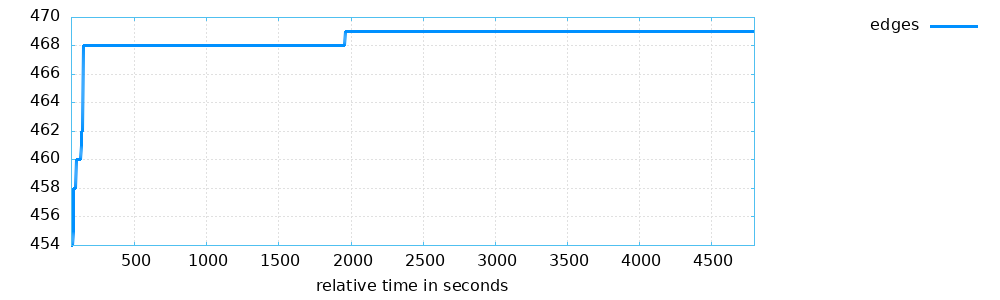
\includegraphics[width=\columnwidth]{plot_output/edges.png}
  \fbox{\rule{0pt}{4cm}\rule{\columnwidth}{0pt}}
  \caption{\texttt{afl-plot} edges graph — instrumented campaign.}
  \label{fig:edges}
\end{figure}

\begin{figure}[h]
  \centering
  % \includegraphics[width=\columnwidth]{screenshots/afl_status_qemu.png}
  \fbox{\rule{0pt}{4cm}\rule{\columnwidth}{0pt}}
  \caption{AFL++ status screen — QEMU-mode campaign.}
  \label{fig:afl-status-qemu}
\end{figure}

\begin{figure}[h]
  \centering
  % 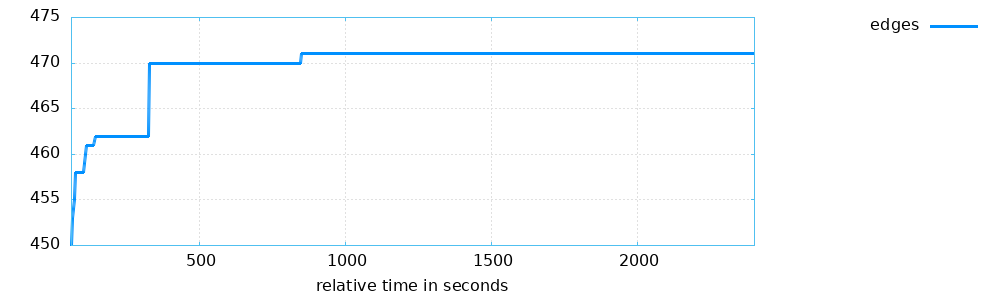
\includegraphics[width=\columnwidth]{plot_output_qemu/edges.png}
  \fbox{\rule{0pt}{4cm}\rule{\columnwidth}{0pt}}
  \caption{\texttt{afl-plot} edges graph — QEMU-mode campaign.}
  \label{fig:edges-qemu}
\end{figure}

%-------------------------------------------------------------------------------
\bibliographystyle{plain}
\bibliography{\jobname}

%%%%%%%%%%%%%%%%%%%%%%%%%%%%%%%%%%%%%%%%%%%%%%%%%%%%%%%%%%%%%%%%%%%%%%%%%%%%%%%%
\end{document}
%%%%%%%%%%%%%%%%%%%%%%%%%%%%%%%%%%%%%%%%%%%%%%%%%%%%%%%%%%%%%%%%%%%%%%%%%%%%%%%%
